% gjilguid2e.tex
% V2.0 released 1998 December 18
% V2.1 released 2003 October 7 -- Gregor Hutton, updated the web address for the style files.

%\documentclass{gji}
\documentclass[referee]{gji}
\usepackage{timet}
\usepackage{gji_extra}
\usepackage{amsmath}
\usepackage{url}

%uncomment for figures
\usepackage{graphicx}

\title[Sp Receiver-Function Sensitivity]
  {The spatial sensitivity of Sp converted waves---Scattered wave kernels
  and their applications to receiver-function migration and inversion}
\author[Mancinelli \& Fischer]
  {N.J. Mancinelli$^1$\thanks{Corresponding author: nicholas\_mancinelli@brown.edu}
  and K.M. Fischer$^1$ \\
  $^1$ Brown University, Providence, Rhode Island, USA.
  }
%\date{Received XXXX December XX; in original form XXXX November XX}
\date{\today}
\pagerange{\pageref{firstpage}--\pageref{lastpage}}
\volume{xxx}
\pubyear{2017}

%\def\LaTeX{L\kern-.36em\raise.3ex\hbox{{\small A}}\kern-.15em
%    T\kern-.1667em\lower.7ex\hbox{E}\kern-.125emX}
%\def\LATeX{L\kern-.36em\raise.3ex\hbox{{\Large A}}\kern-.15em
%    T\kern-.1667em\lower.7ex\hbox{E}\kern-.125emX}
% Authors with AMS fonts and mssymb.tex can comment out the following
% line to get the correct symbol for Geophysical Journal International.
%\let\leqslant=\leq

%\newtheorem{theorem}{Theorem}[section]

\begin{document}

\label{firstpage}

\maketitle

\begin{summary}
We characterize the spatial sensitivity of Sp converted waves to improve constraints on lateral variations in uppermost-mantle velocity gradients, such as the lithosphere--asthenosphere boundary and the mid-lithospheric discontinuities. We use SPECFEM2D to generate 2-D scattering kernels that relate perturbations from an elastic halfspace to Sp waveforms. We then show that these kernels can be well approximated using ray theory, and develop an approach to calculating kernels for layered background models.  As proof-of-concept, we show that lateral variations in uppermost-mantle discontinuity structure are retrieved by implementing these scattering kernels in the first iteration of a conjugate-directions inversion algorithm.  We evaluate the performance of this technique on synthetic seismograms computed for 2-D models with undulations on the lithosphere--asthenosphere boundary of varying amplitude, wavelength, and depth. The technique reliably images the position of discontinuities with dips $<35^\circ$ and horizontal wavelengths $>$100--200~km.  In cases of mild topography on a shallow LAB, the relative brightness of the LAB and Moho converters approximately agrees with the ratio of velocity contrasts across the discontinuities.  Amplitude retrieval degrades at deeper depths. For dominant periods of 4~s, the minimum station spacing required to produce unaliased results is 5 km, but the application of a Gaussian filter can improve discontinuity imaging where station spacing is greater.

\end{summary}

\begin{keywords}
 scattered-wave imaging -- inverse theory -- receiver functions -- computational seismology -- lithosphere--asthenosphere boundary -- mid-lithospheric discontinuity.
\end{keywords}

%My commands
\newcommand{\vp}{v_p}
\newcommand{\vs}{v_s}

\section{Introduction}

When teleseismic body waves encounter gradients in velocity and density structure, the waves scatter into multiple modes that travel at various angles and speeds.  The timing and frequency-dependence of such mode conversions are widely used to infer the depth and sharpness of velocity and density gradients beneath receivers.  Common-conversion point (CCP) stacking---a popular technique analogous to common-midpoint (CMP) stacking from active-source seismology---maps converted phases in a deconvolved seismogram, or receiver function, to a physical position in a model volume by migrating the energy along the converted raypath \citep{Dueker1997}.  This method assumes that structure is locally layered in the vicinity of a seismic converter, such that the converted wave obeys Snell's law.  In practice, however, CCP stacks often reveal dramatic lateral changes in discontinuity depth and sharpness \citep{Lekic2011a, Kind2013, Foster2014, Hansen2015, Hopper2015, Wang2016, Kind2017} thereby motivating the development of methods capable of handling scattering and diffraction effects that are likely important in regions characterized by strong lateral heterogeneity \citep[e.g.,][]{Lekic2017}.

The community has developed several methods to image arbitrarily complex structure with converted teleseisms.  One strategy is to apply poststack migration to the CCP images in order to remove diffraction hyperbolae artifacts \citep{Chen2005}.  A second strategy is to perform prestack migration.  Here a collection of receiver function waveforms are back-projected into model space by summing along lines of constant delay time which have been computed for some assumed background velocity model \citep{Revenaugh1995, Bostock1999, Ryberg2000, Sheehan2000, Poppeliers2003, Frederiksen2004, Cheng2016}.  One variation of this procedure can be expressed as a generalization of slant stacking and hence has become more commonly known as the generalized Radon transform \citep{Bostock2001, Rondenay2005}. Some have approached the problem by solving the Kirchhoff integral for converted waves at an irregular boundary \citep{Levander2005, Wilson2005}, while others have use wave-based reverse-time migration to back-propagate scattered waves to their origin \citep{Shang2012, Shang2017}.

The development of teleseismic migration methods in the late 1990s and 2000s was motivated in part by the increasing popularity of P-to-s (Ps) receiver functions.  Indeed, Ps receiver functions have improved constraints on crustal thicknesses and depths to transition-zone discontinuities, but they often struggle to image gradients at mid-mantle depths, where strong crustal reverberations tend to overprint the weaker signals from more modest velocity gradients in the uppermost mantle.  S-to-p (Sp) conversions, in contrast, do not suffer from this issue and thus have offered a unique glimpse into lithospheric mantle layering structure \citep{Yuan2006}.  Throughout the development of teleseismic migration methods, most attention was applied to Ps conversions, sometimes including information from the back-scattered crustal reverberations.  Given the growing popularity of Sp receiver functions, we are revisiting the topic of teleseimic migration with a particular focus on this subset of converted waves.

The goal of this paper is to characterize the spatial sensitivity of Sp converted waves in order to improve how converted waves image uppermost-mantle velocity gradients, such as the lithosphere--asthenosphere boundary and mid-lithospheric discontinuities.  In Section~\ref{Section1}, we define the sensitivity kernels and how they can be used to obtain an estimate of the spatial distribution of velocity gradients given a set of observations.  We use a numerical approach to generate 2-D scattering kernels that relate perturbations from an elastic halfspace to Sp waveforms. We also develop an approach to approximating the Sp kernels using ray theory, accounting for amplitude information by considering anisotropic scattering patterns and geometrical-spreading effects.
In Section~\ref{Section2}, we test how well lateral variations in uppermost-mantle discontinuity structure are retrieved by implementing these scattering kernels in the first iteration of a conjugate-directions inversion algorithm.  
In Section~\ref{Section3}, we discuss future prospects for applying this method to real datasets and further avenues that could improve the method itself.

\section{SP Sensitivity Kernels}
\label{Section1}

\subsection{Definition}

Fractional perturbations in a model of Earth structure, $\delta \ln{m}$, may be related to amplitudes in the scattered waveforms, $\delta u$, recorded at time $t$, position $\textbf{r}$, and for ray parameter $p$ by integrating against a kernel, $K$:
\begin{equation}
\delta u(t;\textbf{r},p) = \int K(\textbf{s}-\textbf{r},p,t) \cdot \delta \ln{m(\textbf{s})} \, d \, \textbf{s} \,.
\label{eqn:kernel_def}
\end{equation}
$K$ encodes a variety of factors that allow for the imaging of both the strength and location of velocity perturbations within complex 2-D models.  These include (1) wavefield interactions beyond the more typically used P-to-P or S-to-S Fresnel zones, (2) accurate amplitude information from both geometrical spreading and anisotropic scattering patterns, and (3) finite-frequency wavelet information which may allow for the retrieval of sub-wavelength structure.

For the problem of S-to-P converted waves, it is natural to define $u$ as the component of motion aligned with the P-wave polarization for a ray parameter of the incident teleseism.  This can be obtained by applying the free-surface transform \citep{Kennett1991a} if the near-surface velocities and incident ray parameter can be estimated.

\subsection{Comparing Ps and Sp isochrons}

Assuming velocities vary purely in 1-D, a receiver-function amplitude at time $t$ is caused by a change in seismic velocity at some depth $d$, which can be estimated given assumptions regarding the seismic velocities between this converter and the surface. If velocity is allowed to vary laterally, the amplitude at delay time $\delta t$ can be generated by any combination of scatterers along an isochron---a line or surface of constant delay time. The shape of the isochrons, shown in Figure~\ref{fig:isochrons}, can be calculated by using geometrical ray theory to trace the rays through an elastic halfspace originating from a planar wavefront.  The timing of the direct ray is subtracted from the additive timing of the two legs of the scattered ray to obtain a travel time associate with a scatterer at each position.  For P-to-S conversions in an elastic halfspace, these isochrons wrap around the receiver position with either end of the curve terminating at the Earth's surface.  Isochrons for S-to-P conversions, in contrast, bend away from the receiver.  Both $Ps$ and $Sp$ isochrons are skewed towards the direction of the incoming plane wave, with the degree of skewness increasing with ray parameter.

An important difference between the Ps and Sp isochrons can be illustrated by considering how Sp and Ps isochrons behave for very a small delay time $\pm \epsilon$.
At $\delta t=+\epsilon$, Ps receiver functions are only sensitive to structure increasingly near the receiver.  The same is not true for Sp receiver functions: the $\delta t=-\epsilon$ isochron is sensitive to structure at great depths and lateral offsets.

Sp receiver functions tend to have lower signal-to-noise ratios than their Ps counterparts.  While interference from other teleseismic phases and larger signal loss due to attenuation in the parent phase contribute to lower Sp signal-to-noise, differences in kernel structure offer an additional explanation.  Earth structure would need to remain relatively uniform over longer distance scales to produce constructive interference along Sp isochrons, relative to Ps isochrons.

\subsection{Spectral-element calculations}

Moving beyond the timing information contained in isochrons, we turn to spectral-element simulations to model wave-propagation through a suite of simple models with small, weak circular scatterers.  Later, we will use these calculations to benchmark a computationally efficient approach to kernel computation based on ray theory. 

Here we present sensitivity kernels which relate the strength and polarity of an arbitrarily small and weak scatterer (i.e., such that the Born approximation is valid) in a 2-D field to the daughter amplitude recorded at the specified time.  For the spectral element calculations, we used software package SPECFEM2D 7.0.0 \citep{Tromp2008, specfem2dsoftware} published under the CeCILL v2 license.  We ran a series of forward models with a weak ($\delta \ln \vs = 1\%$) small (2.5~km radius) scatterer at varying depths (Figure~\ref{fig:ModelSetup}).  We repeated this process for a variety of scatterer depths and plane-wave incidence angles to populate the kernel.  To reduce the number of free parameters, we set $d\ln v_p=d\ln v_s$ and $d\ln \rho =0$.

Upon each successive simulation, the scatterer was translated vertically by 5~km to populate the kernel across depths from 0--300~km. We placed a linear array of 150 receivers at the free surface, situated 1350 to 2100 km from the left edge of the domain.  To populate the kernel elements along the ray-parameter dimension, we ran simulations for a variety of plane-wave angles---23, 25, 27, 29, 31, and 33~degrees---which corresponds to the typical range of ray parameter used in $Sp$ receiver function studies.

The spectral elements were spaced 2 km in the vertical and horizontal dimensions.  Each of these elements contained 5 mesh points in both directions, resulting in an effective uniform mesh spacing of 400 m.  The domain of each model---3000 km wide by 1500 km tall---was chosen to minimize edge effects.  In other words, we set the model domain to be sufficiently large so that reflections from model edges were avoided in the time windows of interest.

In this paper we present kernels computed for Ricker-wavelet plane waves with dominant periods of 4 and 8~s, but one could use an identical setup to compute kernels for waves with other dominant periods and pulse shapes.  Of course, simulating wave propagation at shorter periods is hindered by the requirements of finer mesh spacing and shorter time steps, but pushing this limit is not necessary for the study of Sp waves, as actual observations tend to exhibit dominant periods of 4 seconds or greater, owing to the attenuation of high-frequencies experienced by teleseismic shear waves.

These models are simple: they assume half-space velocities, an unperturbed and planar incident wavefield, and are limited to purely 2-D structure.   A single serial simulation---run on compute nodes at the Brown University Center for Computation and Visualization
\footnote{See \url{https://www.ccv.brown.edu/technologies/computing}
for hardware specifics.}
---took approximately 9~hours to run on a single processor with an allocation of 8~GB memory.
A single simulation populated the kernel in both the time and horizontal distance dimensions, but to populate the kernel in the depth (60 points) and ray-parameter dimensions (5 points), we ran $\sim 300$ separate simulations in parallel for a total of $2250$ core-hours.

An advantage of our model setup is that it is identical to the setup used to generate the synthetic data that we used to illustrate the utility of these kernels at the end of this paper.  When applying these concepts to true teleseismic data, using a curved incident wavefront is, of course, preferred.  A following section will outline how kernels can be computed by relaxing these assumptions.

\subsection{Kernel characteristics}

\subsubsection{Amplitude and polarity}

The amplitudes of the Sp sensitivity kernels are null along the direct raypath (Figure~\ref{fig:KernelsTime}).  As one moves away from the raypath, the absolute amplitudes rapidly increase to a peak value and slowly decay.  At large offsets, this decay goes as the inverse square-root of the distance---the theoretical decay from geometrical spreading in 2-D.  The amplitude and polarity information are consistent with the analytic scattering pattern for S-to-P \citep{Wu1985, Bostock1999, Rondenay2009, Sato2012}, which predicts a null amplitude for a scattering angle of zero (i.e., along the ray) and flipped polarities on opposing sides of the ray.  The rapid increase in amplitude close to the raypath is explained by the scattering pattern term, whereas the gradual decrease in the kernel envelope away from the raypath is dominated by geometrical spreading.

\subsubsection{The finite-frequency wavelet}

Computing the kernel in this way naturally incorporates finite-frequency effects.  The primary effect of finite-frequency waves in this context is the broadening of the sensitivity in directions locally perpendicular to the isochrons (Figure~\ref{fig:KernelsPeriod}).  We also note that the scattered wavelet appears to be phase shifted by $\pi/4$ from the incident wavelet.  In fact, the SEM calculations conducted for different periods show that the scattered wavelet is well described as the one-and-one-half derivative of the source wavelet with an additional Hilbert transform applied.  In the frequency domain this set of operations may be expressed as a multiplication by the frequency dependent factor
\begin{equation}
\label{eqn:FrequencyFactor}
\Psi(\omega) = -\omega^2 \sqrt{\frac{1}{-i\omega}} \, .
\end{equation}
This factor is present in the perturbed Green's tensor derived using Born's approximation in 2-D \citep{Bostock1999}, and the $\pi/4$ phase shift is consistent with the far-field displacement for a point source (or point scatterer, in this case) in 2-D \citep[e.g.,][]{Frazer1980, Hudson1980}.

\subsection{Rapid computation using ray theory}

In addition to computing the kernels numerically and identifying their salient features, we developed an efficient and accurate means to generate them using ray theory. This approach is orders of magnitude faster than the spectral-element approach, taking a few core-minutes to complete.  For the 2-D case, an element of the kernel can be described by four indices: two for position $r_{ij}$, one for delay time $t_k$, and one for ray parameter $p_l$.  Each element of the kernel was obtained by multiplying three factors
\begin{equation}
\label{eqn:KernelRayTheory}
K^\prime (r_{ij},t_k,p_l) = W(r_{ij},t_k,p_l) \, A^G(r_{ij}) \, A^S(r_{ij})
\end{equation}
where $W$ is the timing--wavelet term, $A^G$ is the geometrical spreading term, and $A^S$ is the scattering amplitude term (Figure~\ref{fig:KernelPieces}).

\subparagraph{Timing--Wavelet Term}
The term $W(r_{ij},t_k,p_l)$ (Figure~\ref{fig:KernelPieces}c,g) was computed by tracing rays through an assumed background velocity structure. The timing of the scattered arrival was computed by tracing an upgoing S ray from a reference teleseismic wavefront (approximated by a straight line whose slope is determined by the ray parameter) upwards until it reached the scatterer.  Then an upgoing P ray was traced from the scatterer to the receiver.  The delay time was obtained by subtracting from this Sp time the time of an upgoing S phase for a ray directly between the reference teleseismic wavefront and the receiver.  Our subroutine can currently handle layered velocity models, but in principle one could apply 2- or 3-D raytracing algorithms to compute isochrons for higher-order velocity models.

In practice it was not trivial to trace a ray between two points.  The problem can be stated as: given two points $r_{i}$ and $r^\prime_{i}$, with $r^\prime_{3}<r_{3}$ and $r^\prime_{1} \ge r_{1}$, find the ray parameter, $p$, that defines the ray connecting with the two.  Subscript 1 denotes the lateral dimension whereas subscript 3 denotes depth (positive downward).  This problem can be solved by tracing rays for a range of ray-parameters, $p_j$, and recording the horizontal distance $\Delta x_j$ traveled by each.  For the simple velocity models considered in this study, increasing $p_j$ always yielded a larger value of $\Delta x_j$, so the values of $\Delta x$ above and below the target ($r^\prime_1-r_1$) could be interpolated to obtain a unique estimate for $p$.  This approach worked fairly well in practice when spraying 1000 discrete rays at incidence angles $\theta_j$ between 0 and 90 degrees (where the incidence angle is defined by $p_j=\sin{\theta_j}/\alpha$), but for large incidence angles uniform spacing along the range of $\theta_j$ yielded unstable results.  A modified spacing where increments $\cos{\theta_j}$ were uniformly spaced gave finer resolution in $\theta_j$ at large incidence angles, and thus improved the method's stability. Considerable speedup was achieved for some pairs of points by using Newton's method to find the root of
\begin{equation}
\Delta x (p) - (r^\prime_1-r_1) = 0 .
\end{equation}
In brief, two rays were traced upward for two values of ray parameter, $p_0$ and $p_0+\delta p$, to obtain a local estimate for $\Delta x (p_0)$  and $d \Delta x (p_0) / dp$.
Then, the ray parameter was updated using
\begin{equation}
p_{1}=p_0-\frac{\Delta x (p_0)-(r^\prime_1-r_1)}{ d \Delta x (p_0) / d p}
\end{equation}
and the process was repeated until convergence.

In order to compare these ray-theoretical kernels with those computed from SPECFEM, we took the second derivative of a Gaussian pulse of an appropriate width to form a Ricker wavelet.  An additional one-and-one-half derivative and a successive Hilbert transform was required to achieve the $\pi/4$ phase shift that occurs for waves emanating from a point source in 2-D \citep{Hudson1980, Bostock1999}.  In practice, the wavelet shape can take the form of our choosing.  For the test cases shown in the next section, for example, we set the wavelet shape to be a narrow-peaked Gaussian, and instead we apply the $\pi/4$ phase shift and filters to the waveforms before inversion.

\subparagraph{Geometrical Spreading Term}  $A^G(r_{ij})$ (Figure~\ref{fig:KernelPieces}b,f) was calculated by tracing rays through the background velocity structure and taking the square root of the energy density:
\begin{equation}
A^G=\sqrt{\tilde E}
\end{equation}
with
\begin{equation}
\tilde E=\frac{1}{2\pi} \left| \frac{dp}{dx} \right| \frac{1}{\cos\theta_1 \cos\theta_2 \, u_1}
\end{equation}
where $dp/dx$ is the change in ray parameter with respect to horizontal distance, $\theta_1$ and $\theta_2$ are the angles of incidence at the scatterer and the receiver, and $u_1$ is the slowness. This expression reduces to
$
\sqrt{\frac{1}{2\pi r}}
$
in the case of an elastic halfspace (Figure~\ref{fig:KernelPieces}b), in accordance with the theoretical prediction.

\subparagraph{Scattering-Amplitude Term} For S-to-P conversions from a point scatterer, the angular dependence of the scattered wave amplitude depends upon the angle between the incident and scattered rays $\phi$ and is given by
\begin{equation}
\begin{split}
A^S= 
 &  \frac{ \delta \beta}{\beta_0} \left( 2  \frac{\beta_0}{\alpha_0} \sin{2\phi_{ij}} \right) \\
- & \frac{ \delta \rho}{\rho_0} \left(\sin{\phi_{ij}} + \frac{\beta_0}{\alpha_0}  \sin{2\phi_{ij}} \right)
 \end{split}
\end{equation}
where $\rho_0$, $\alpha_0$, and $\beta_0$ are density, P-wave velocity, and S-wave velocity from the background model, respectively \citep{Bostock1999}.  To calculate the Sp sensitivities to velocity, we set 
\begin{equation}
\frac{ \delta \beta}{\beta_0}=0.01
\end{equation}
and
\begin{equation}
\frac{ \delta \rho}{\rho_0}=0 \,  .
\end{equation}
Doing such sets the kernel units to velocity perturbations in percent, and discards contributions from density perturbations (Figure~\ref{fig:KernelPieces}a,e).

\subparagraph{Free-Surface Transform}
As a final step, we projected $K^\prime$---which contains the scalar amplitude information---onto the radial and vertical components, and used the free-surface transfer matrix to obtain $K$, the sensitivities for the component of motion aligned with the $P$-wave polarization, as in Equation~\ref{eqn:kernel_def}.

\subsection{Half-space versus layered background models}

The two columns in Figure~\ref{fig:KernelPieces} compare the kernel terms computed for a half-space versus those computed assuming a three-layer background model. The jumps in the scattering pattern contours in Figure~\ref{fig:KernelPieces}e  are caused by the changes in angle required to satisfy Snell's law across layers of different velocity.  The region of enhanced amplitude reduction due to geometrical spreading beneath the Moho exists in Figure~\ref{fig:KernelPieces}f,h because $dp/dx$ becomes very small for the rays connecting those points with the receiver.  Another way to think about this is that $dp$ must become increasingly fine for equal increments of $dx$ as the critical ray parameter of the upper medium is approached.  The weaker amplitude reduction beneath the LAB is due to the change in incidence angle as the ray crosses from the slow asthenosphere to the fast lithosphere.  The slight bends in the timing--wavelet term in Figure~\ref{fig:KernelPieces}g match those computed for isochrons.

\subsection{Equivalence}

As a demonstration of the accuracy of the ray-theoretical kernels, we compared them with those computed directly from the spectral-element method for a Ricker wavelet with a dominant period of 8~s in the case of an elastic halfspace (Figure~\ref{fig:KernelEquivalence}, upper and center row). The shapes of the ray-theoretical kernel are virtually indistinguishable from those derived from SPECFEM.  The middle zero-crossing of both kernels agrees with the isochron curve (dotted black line, Figure~\ref{fig:KernelEquivalence}).  This excellent consistency validates the ray-theoretical kernels, including the frequency dependence of $\omega^{1.5}$, which is accounted for in Equation~\ref{eqn:FrequencyFactor}.

To test how closely the amplitudes agree, we plotted the mean absolute amplitude at each offset, and we inverted for an optimal scaling factor to determine by how much the SEM kernel is larger than the ray-theoretical one\ (Figure~\ref{fig:KernelEquivalence}, lower row).  We found that the SEM kernel amplitudes to be $9.9\pm0.5$ percent larger than those derived from ray-theory. Meshing inaccuracies provide the most likely reason for this discrepancy; the ideal small circular scatterers in our input model file are somewhat enlarged once interpolated onto the rectilinear mesh over which the SEM simulation is carried out and thus yield amplitudes slightly larger than expected.

\section{Imaging undulations on the lithosphere--asthenosphere boundary}
\label{Section2}

\subsection{Synthetic data}

Next we demonstrate the usefulness and applicability of these sensitivity kernels by solving for a heterogeneous Earth model given a set of scattered waveforms.
In particular, we explored how kernel-based imaging with synthetic Sp phases can resolve negative velocity gradients at uppermost-mantle depths such as the lithosphere--asthenosphere boundary and the mid-lithospheric discontinuity.

To generate ``data'' for these imaging experiments, we used SPECFEM2D to simulate teleseismic wave propagation through models of the uppermost mantle containing negative velocity gradients with lateral variations.  For all models, the crustal upper layer was 60-km thick with uniform elastic parameters defined by $\alpha=5.66$~km/s, $\beta=3.20$~km/s, and $\rho=2.80$~g/cc.  The mantle lithosphere directly beneath the Moho was of variable thickness with typical uppermost mantle velocities: $\alpha=7.92$~km/s, $\beta=4.40$~km/s, and $\rho=3.3$~g/cc.  The bottom layer---with $\alpha=7.28$~km/s, $\beta=4.04$~km/s, and $\rho=3.3$~g/cc---had slightly slower velocities characteristic either of the asthenosphere beneath young lithosphere or of potentially volatile-rich mid-lithosphere in cratons.  To simplify the following discussion, this discontinuity will hereafter be referred to as the LAB, but these results could just as well be applied to the MLD.

We prescribed topography on the LAB as a sinusoidal variation with average depth $d$, trough-to-peak height $h$, and wavelength $\lambda$.  There was no topography on the free-surface or the Moho.  We varied $d$ from 120--180~km; $h$ from 0--40~km; and $\lambda$ from 100--800~km.

The incident teleseisms were locally simulated as a plane-wave.  The source-time function was a Ricker wavelet with a dominant period of 4~s.  A linear array of 150 receivers was placed at the free surface, with an aperture of 650~km and an inter-station spacing of $\sim5$~km.  The structure was illuminated by four plane waves propagating from left to right at angles of 23, 26, 29, and 32 degrees from horizontal, and four plane waves propagating from right to left at the same angles.  Structure was designed to be symmetric about the midpoint of the array so that the simulations with right-to-left propagating teleseisms did not have to be computed.  

\subsection{A back-projection approach}

We addressed the linear geophysical inverse problem using a back-projection approach:
$$
\hat{ \textbf{m}} = \textbf{G}^T \textbf{d}
$$
where $\hat{ \textbf{m}}$ is the estimate of structure, $\textbf{d}$ is a vector containing all of the scattered waveforms, and $\textbf{G}$ is the matrix relating the two using appropriately arranged interpolants of the Sp sensitivity kernel.
Rather than attempting to invert $\textbf{G}$ directly, we preformed the first iteration of a conjugate--gradients inversion by projecting $\textbf{d}$ into the model space by applying the adjoint operator, the transpose $\textbf{G}^T$.

To prepare the data vector, we applied the free-surface transform to the radial and vertical components of the synthetic seismograms to obtain waveforms aligned with the SV and P polarizations.  The SV, or parent, component pulses were deconvolved from the P, or daughter, waveforms to yield a set of receiver functions.  A half-derivative was then performed on each receiver function to achieve a $\pi/4$ phase shift, which can be done in the frequency domain by multiplication with $(i\omega)^{1/2}$, where $\omega$ is the angular frequency.  The effect of this half-derivative is to phase shift the synthetic data so that discontinuities are highlighted by phase pairs, with a positive phase shallower and a negative phase deeper for velocity increases with depth, and a negative phase shallower and a positive phase deeper for velocity decreases with depth (Figure 6).  Application of a 1.5-derivative would center a negative phase on a velocity increase and a positive phase on a velocity decrease, but also generates more unwanted side-lobe energy in the image.  To be clear, the 1.5 integral operator is the true adjoint in the context of this back-projection problem, but we found that procedure to be unstable when applied to our synthetic data.  Therefore, we instead achieved the $\pi/4$ phase shift by applying the more-stable half-derivative operator, while introducing the caveat that the frequency dependence is no longer accounted for in this context.  This is not problematic, however, if only relative amplitudes in the image are considered.

To calculate the $\textbf{G}$ matrix, we defined a reference background structure with a 60-km thick crust, a 60-km thick mantle lithosphere, and a 180-km thick asthenosphere.  The corresponding velocities and densities were identical to those used in the spectral-element calculations.  In this back-projection example, we set the time--wavelet term of Equation~\ref{eqn:KernelRayTheory} to be a narrow-peaked Gaussian centered on each isochron.

\subsection{Ideal data coverage}

Over the course of the synthetic experiments, a station spacing of 5~km produced minimal aliasing in the back-projection images. Figure~\ref{fig:LABStructures} shows several examples of relatively good recovery of LAB undulations given 5 km station spacing, while Figure~\ref{fig:BadExamples} illustrates cases that failed.

Over the range of models tested, the positions of Moho and LAB discontinuities are accurately recovered in cases where the half-wavelength of the LAB undulations divided by the trough-to-peak amplitude is less than about $1/5$, or rather, undulations with a maximum dip of $\sim35^\circ$ (Figure~\ref{fig:LABStructures}).  This significantly exceeds the performance of Sp CCP stacking, which reliably recovers discontinuities only when they dip at angles of  $<10^\circ$ to $15^\circ$ \citep{Lekic2017}.

For discontinuity undulations that exceed dips of $>35^\circ$, two behaviors occurred:
\begin{enumerate}
\item For the case of large trough-to-peak topography $>$10--20~km, the peaks and troughs are imaged as bright converters but little, if any, energy sums coherently to illuminate more steeply-dipping segments (Figure~\ref{fig:BadExamples}, upper and middle panels).  This is likely due to the sub-horizontal shape of the Sp kernels, which is better suited for imaging horizontal structure.
\item For the case of short ($\sim 100$~km) wavelength topography, the lateral variations are so fine that the finite wavelength of depth-migrated phases cannot resolve the structural variations even when the amplitude of the topography is mild (Figure~\ref{fig:BadExamples}, lower panel).  Instead, energy is smeared in the vertical direction, and the resulting image does not clearly retrieve the fine-scale undulations.  The wavelength of these undulations is approximately three times that of the P wavelength.  It is likely that the sub-horizontal shape of the Sp isochrons preclude lateral imaging down to the wavelength scale.
\end{enumerate}

Uncertainties in discontinuity depth retrieval can be estimated by measuring across the image the residuals of the retrieved zero-crossing of a given phase with respect to the true depth of the discontinuity.  In Figure~\ref{fig:LABStructures} (top-left) for example, the RMS residual in depth is 1.00~km for the Moho interface, and 0.80~km for the undulating LAB interface.  The RMS residual becomes slightly larger if (1) the topography wavelength is decreased; (2) the topography amplitude is increased; or (3) the discontinuity interface is moved to greater depth.  Nevertheless, the largest RMS residuals are on the order of 1~km for the Moho and 2--3~km for the LAB.  Increasing the station spacing can also increase uncertainties.  For most geometries depicted in Figure~\ref{fig:LABStructures}, this increase is relatively minor, but in the case of larger amplitude topography (e.g., lower-left panel in Figure~\ref{fig:LABStructures}) increasing the station spacing from $\sim 5$ to $\sim 20$~km increased the RMS residual of the LAB interface from 2.96 to 9.08~km.

The accurate retrieval of undulation position does not appear to depend much upon depth, despite keeping the assumed discontinuity depth at 120~km in the ray tracing model.  However, the imaged amplitude of the 180-km LAB discontinuity is somewhat weaker than the equivalent discontinuity at 120~km.  For a wavelength of 400 km and trough-to-peak topography of 10~km, for example, the image of the deeper discontinuity is reduced in amplitude by $\sim 50$\%.  There is also variation in converter brightness with offset.  The converters tend to be brightest at the center of the image, where model nodes are most optimally illuminated by the data.  These lateral variations in brightness are typically less than 10\% beneath the array, but outside of the array the apparent converter amplitudes can become dramatically reduced.  That being said, the steep incidence of S-to-P converted waves allow the back-projection images to recover a relatively accurate semblance of deeper LAB topography well outside of the array.

\subsection{Suboptimal data coverage---the role of smoothing}

In cases where station spacing exceeds 5~km, aliasing becomes visible in the images (Figures~\ref{fig:LABStructures10km} and ~\ref{fig:LABStructures20km}).  This appears as energy smearing along isochrons.  At 10-km station spacing, aliasing is visible, but its amplitude is sufficiently weak that it is unlikely to be problematic in practice. At 20-km spacing, however, the amplitudes are aliased to proportions comparable to the scattering potential amplitude of the Moho and LAB interfaces.

This type of aliasing occurs when the dominant period of the data is small and the station spacing is large, such that receiver functions at neighboring stations do not destructively interfere when back-projected to model nodes.  This can be addressed by applying a low-pass filter to the receiver functions to increase the dominant period.  In Figure~\ref{fig:StationSpacing} we apply a Gaussian low-pass filter that introduces no additional sidelobes. Because broadening the waveforms in this way smears the energy around the discontinuities in the resulting image, there is a tradeoff between damping the aliased energy and resolution.

\section{Discussion and Future Work}
\label{Section3}

\subparagraph{How important is an accurate reference model?}
The position of the 180~km LAB is well-retrieved despite assuming a 120~km LAB depth in the ray-tracing model.  In a more extreme test, where we assumed a uniform halfspace ray-tracing model with lithospheric velocity and density parameters, we found that the discontinuity positions were vertically offset by $\sim10$~km.  Hence we conclude that for optimal results the reference model should attempt to include an accurate estimate of crustal thickness, but modest ($<10\%$) fractional variations in velocity in the uppermost mantle do not result in significant mismapping of energy.

\subparagraph{The physical meaning of scattering potential}

From the equations laid out in Sections~\ref{Section1}~and~\ref{Section2}, it is evident that scattered-wave amplitude is linear with respect to perturbations in velocity and density according to this theory.  To test how well this holds up in the back-projection images, we measured the amplitude contrasts across the Moho and LAB in each column of our synthetic back-projection experiments, and compared that ratio to the ratio of velocity perturbations in the input models (Figure~\ref{fig:FigureRecovery}).

For the most moderate (i.e., least topography and longest wavelength) LAB undulations we tested at a depth of 120 km, the median amplitude contrast ratio in the back-projected image is $<15$\% weaker than the theoretical value.  There is, however, considerable spread in the ratio across the image because both converters, the LAB in particular, independently fluctuate in brightness.  We note that the largest amplitude contrasts in the image do reach and sometimes exceed the expected ratio.

When the LAB undulations are more extreme, the retrieved amplitude contrasts across the LAB become significantly smaller than the input velocity contrast, as would be expected when the interface is less well imaged.  Likewise, when the LAB is at a depth of 180 km, the LAB amplitude contrasts are weaker than those for the 120-km depth case, even when the amplitude of LAB topography is mild.  We interpret this as a limitation imposed by the aperture of this array; at greater depths the model points are not as well sampled as those at intermediate depths \citep[c.f.,][]{Rondenay2005}.

Another factor not accounted for in these back-projection experiments is how the amplitude of the parent pulse is affected by passing through heterogeneity. The Born approximation treats the data as a sum of the incident (parent) and scattered (daughter) wavefields, but in reality the parent wavefield is modulated by the interfaces through which it passes.  This limitation could be addressed in future work by applying the appropriate set of transmission coefficients to the parent and daughter pulses.

Finally, we note that the back-projection operator does not generally yield a model which, when operated on by $\textbf{G}$, gives a perfect match to the data, and it is possible that the amplitudes at greater depths are less-well retrieve because of the use of this operator.  Future work will explore how conjugate-direction schemes could improve the accuracy of the retrieved amplitude information.  Using the inverse of the Hessian matrix instead of the back-projection operator is an another promising approach that may work well with small datasets.

\subparagraph{Comparison with other studies}
The kernels derived in this paper differ substantially from the weighting functions typically used to smooth CCP stacks \citep[e.g.,][]{Lekic2017}.  These weighting functions are typically strongest along the ray---in contrast to these kernels which are null along the ray---and decay relatively rapidly far from the ray. We emphasize that these results indicate that structures well outside of the weighting function can contribute to the observed $Sp$ amplitude at any delay time.

In this paper we have chosen to characterize Sp sensitivity kernels for scattered-wave amplitudes with respect to scatterer position.  An alternate formulation has been proposed to relate Ps sensitivities of scattered-wave phase to perturbations in discontinuity depth \citep{Deng2015}.  Such a formulation requires \emph{a priori} knowledge of mean discontinuity depth and the velocity/density contrasts across so it is well suited for targeting ubiquitous discontinuities.  Our approach, by contrast, does not rely on such knowledge and thus is better suited for imaging laterally variable discontinuities such as the LAB and MLD.

It is difficult to draw direct comparisons between the method we have outlined and other teleseismic migration schemes \citep[e.g.,][]{Revenaugh1995, Bostock1999, Ryberg2000, Sheehan2000, Poppeliers2003, Frederiksen2004, Cheng2016} because most previous work focused on Ps conversions, whose kernels average over different orientations of heterogeneity than those presented here.  It appears that in general it is more challenging to image steeply dipping structure with Sp conversions than it is with Ps conversions, owing to the sub-horizontal shape of the Sp isochrons versus the more circular shapes of the Ps isochrons.  One similarity that we do expect is that volume resolution of Sp back-projection is proportional to frequency, as is true for the P-to-s case \citep{Rondenay2005}.  For Ps migration methods, horizontal resolution is thought to be inversely proportional to scatterer depth \citep{Poppeliers2003}.  Our Sp back-projection experiments, however, do not indicate a strong decrease in dip resolution with depth. Rather, at greater depths the amplitude swings become weaker regardless of dip.

\section{Conclusions}

We have characterized the spatial sensitivity of Sp converted waves in a half-space using spectral element simulations, and we have formulated a ray-theoretical method for calculating Sp sensitivities in uniform and layered models.  The shapes of the frequency-dependent kernels generated using these complementary methods agree well, and their amplitudes match to within 10 percent.  

Back-projection experiments show that lateral variations in uppermost-mantle discontinuity structure can be retrieved by implementing these scattering kernels.  We have evaluated the performance of this technique using synthetic seismograms computed for 2-D models with undulations on the lithosphere--asthenosphere boundary of varying amplitude, wavelength, and depth. For dominant periods of ~4 s, we have placed constraints on the minimum resolvable lateral wavelength of LAB topography ($>$100--200~km), the maximum resolvable dip angle ($<35^\circ$), and the minimum station spacing (5--10 km) required to produce unaliased results.

Concurrent, but independent, work by \citet{Hansen} is striving to develop scattered-wave kernels for multi-mode conversions with ray-tracing through laterally inhomogeneous velocity models.  Our future work will apply these approaches to teleseismic datasets and extend them to 3-D imaging. 

\begin{acknowledgments}

For providing access and support for SPECFEM2D, we owe gratitude to the Computational Infrastructure for Geodynamics (http://geodynamics.org) which is funded by the National Science Foundation under awards EAR-0949446 and EAR-1550901. This research was conducted using computational resources and services at the Center for Computation and Visualization, Brown University.
Funding for this research was provided by the NSF EarthScope Program  under award EAR-1614066.
We thank two anonymous reviewers for their constructive comments.

\end{acknowledgments}

\bibliographystyle{gji}
\bibliography{mendeley}

\bsp % ``This paper has been produced using the Blackwell
     %   Publishing GJI \LaTeXe\ class file.''

\newpage

\begin{figure}
\centering
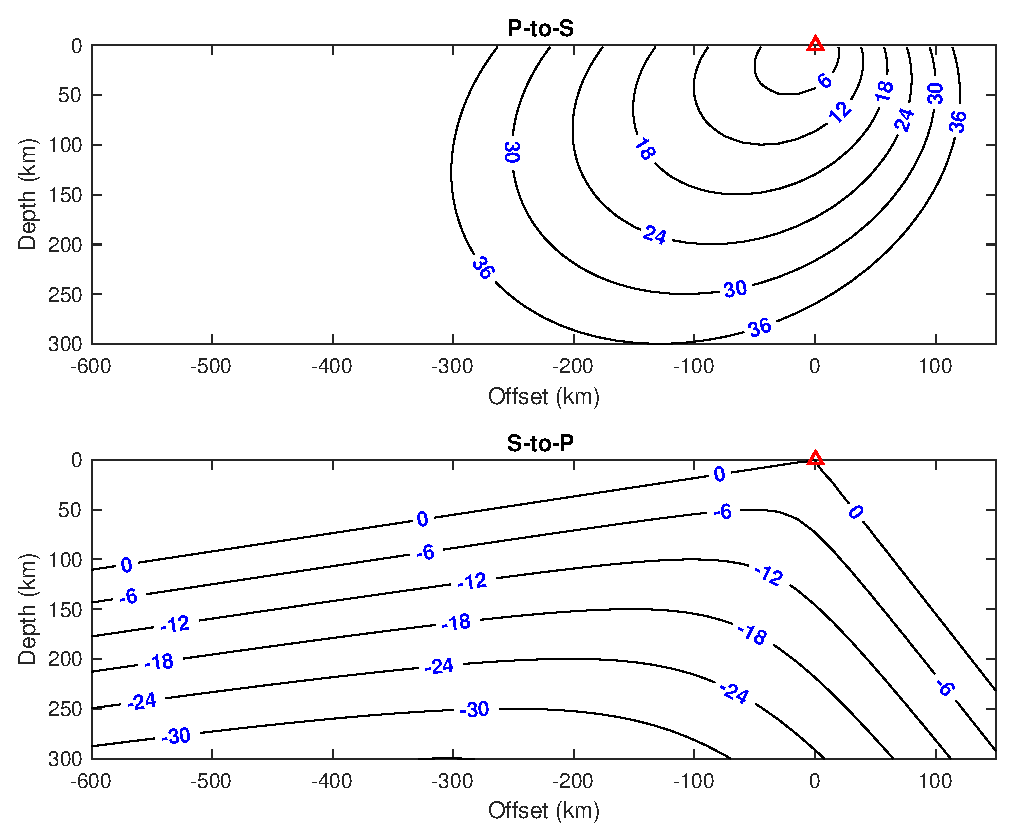
\includegraphics[]{img/figure1.eps}
\caption{Delay time isochrons (in seconds) for Ps (upper panel) and Sp (lower panel) converted waves for a station at the surface (red triangles) above an elastic half space with $\vp=7.92$~km/s and $\vs=4.4$~km/s. Contours are plotted for travel times between at increments of 6~s.  These isochrons are calculated for an incident plane wave propagating from left to right at an angle of 25~degrees from the horizontal.}
\label{fig:isochrons}
\end{figure}

\begin{figure}
\centering
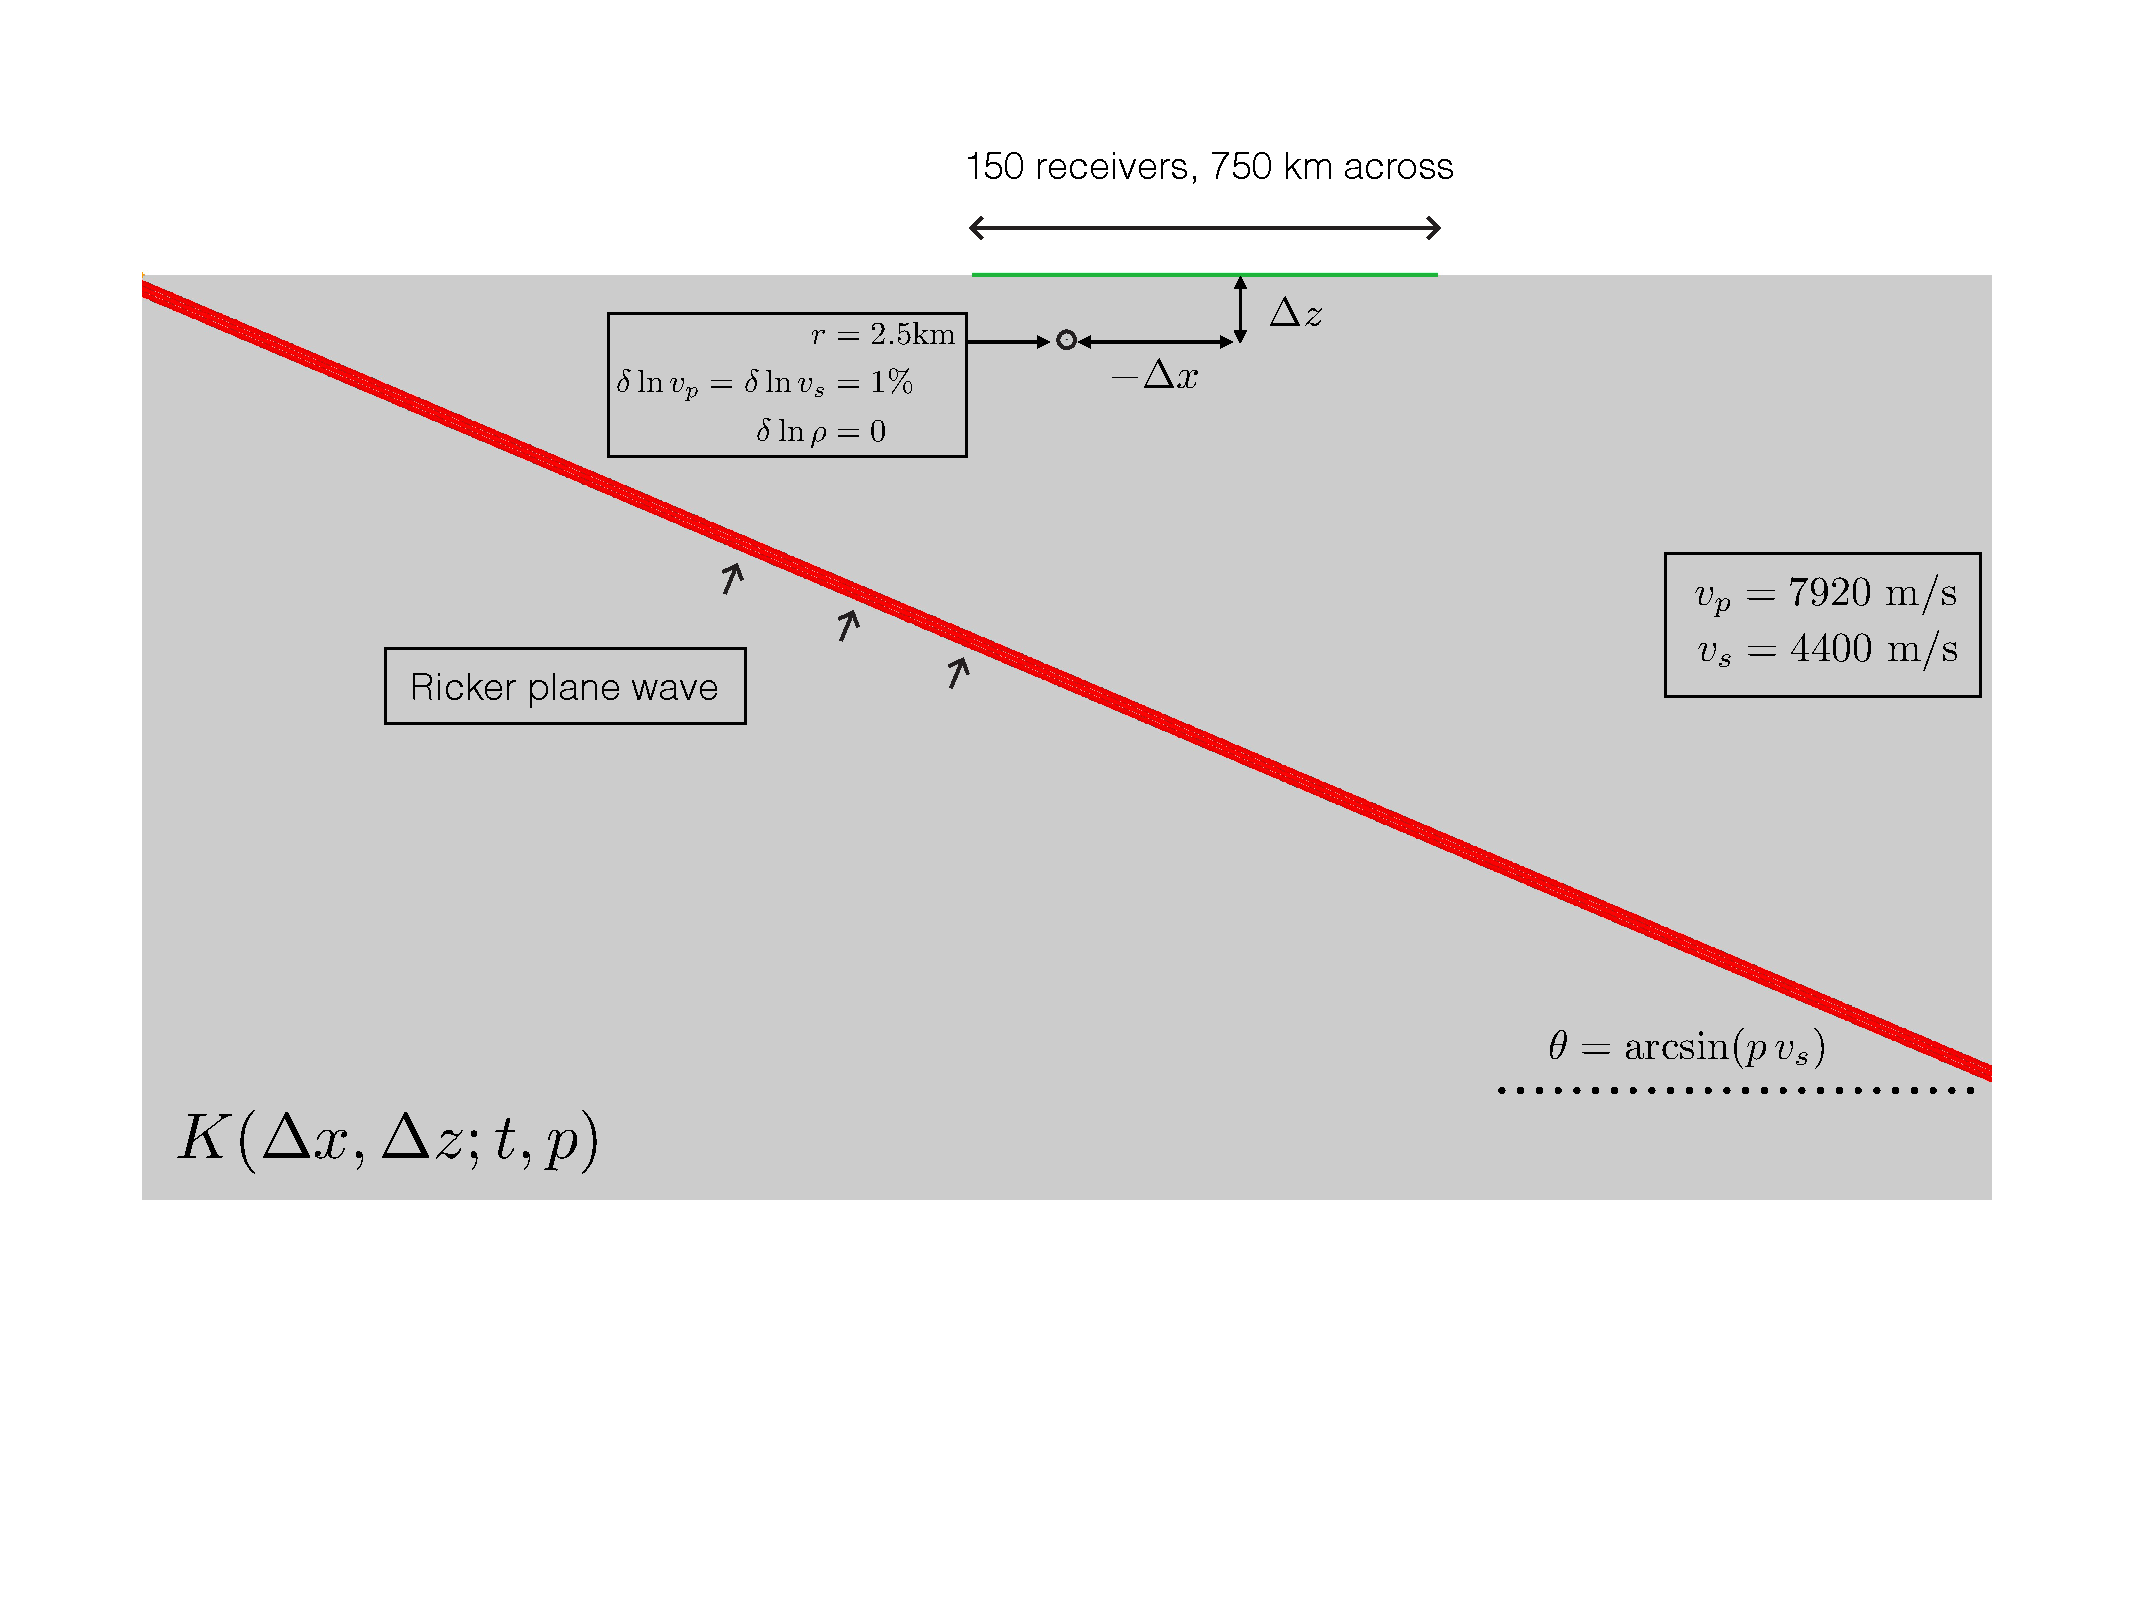
\includegraphics[scale=0.5]{img/Figure2.pdf}
\caption{Annotated setup for a SPECFEM2D simulation.  One simulation populates the kernel at all offsets (one discrete measurement per station) and all delay times.  Many simulations are required to populate the kernel as a function of depth and incidence angle.}
\label{fig:ModelSetup}
\end{figure}

\begin{figure}
\centering
\includegraphics[]{img/figure3.eps}
\caption{Sp converted wave sensitivity in an elastic halfspace ($\vp=7.92$~km/s and $\vs=4.4$~km/s) derived by spectral-element simulations.  The top three panels show sensitivities for a incident ray with horizontal slowness of 0.078~s/km at delay times of -23.8~s, -15.8~s, and -7.8~s. The lower three panels show sensitives at delay time of -15.8~s, for incident waves with horizontal slownesses of 0.059, 0.078, and 0.096~s/km (corresponding to wavefronts oriented 15, 20, and 25 degrees from the horizontal).  The red triangle shows the location of the receiver from which relative distances are calculated.  The incident plane wave---a Ricker wavelet with a dominant period of 8 seconds propagated across the model plane from left to right.  In all panels, areas shaded in red correspond to locations where perturbations generate amplitudes of the same sign, whereas areas shaded in blue correspond to locations where perturbations generate amplitudes of the opposite sign.  Red triangles mark the locations of the station for which the kernels are calculated.}
\label{fig:KernelsTime}
\end{figure}

\begin{figure}
\centering
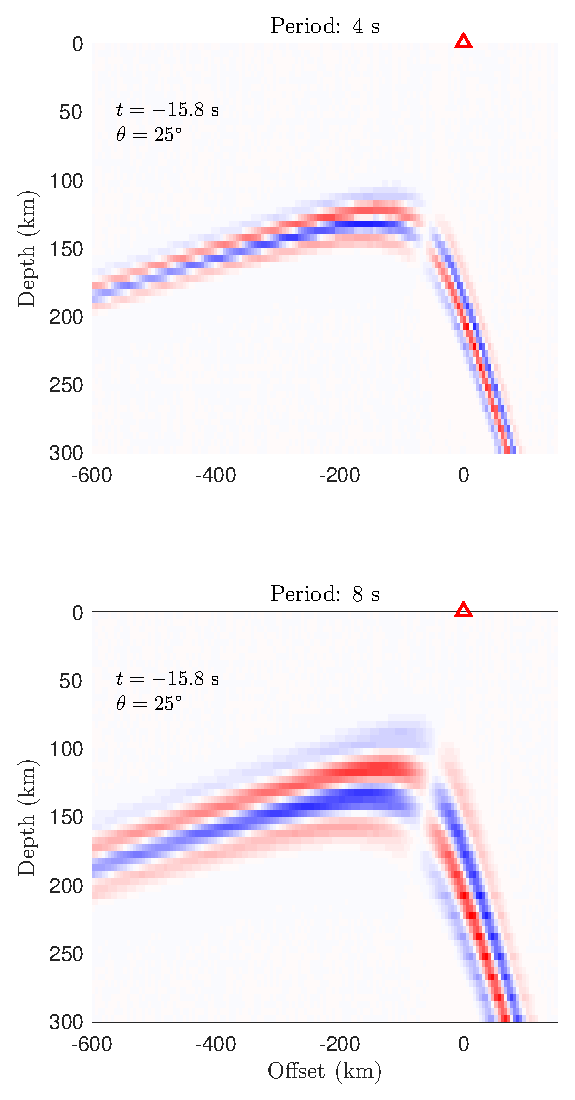
\includegraphics[]{img/figureFrequencyDependence.eps}
\caption{The frequency dependence of Sp sensitivities.  The setup parameters are the same as in Figure~\ref{fig:KernelsTime}, but the upper panel shows a kernel computed for a dominant period of 4 s and the lower panel shows a kernel computes for a dominant period of 8 s. Red triangles mark the location of the station origin in each panel.}
\label{fig:KernelsPeriod}
\end{figure}

\begin{figure}
\centering
\includegraphics[scale=0.8]{img/figure4.eps}
\caption{Contributing factors to sensitivities computed using ray theory. (a) Angular dependence of the scattering pattern for an elastic halfspace; (b) Geometrical spreading term for an elastic halfspace; (c) Time-wavelet term for an elastic halfspace; (d) The element-wise product of (a), (b), and (c); (e-h) Same as a-d for a layered background velocity model with a slow crust ($\vs = 3.2$~km/s ) on top of a fast lithospheric mantle ($\vs = 4.4$~km/s) overlying a relatively slow asthenosphere ($vs=4.05$~km/s).}
\label{fig:KernelPieces}
\end{figure}

\begin{figure}
\centering
\includegraphics[]{img/figure5.eps}
\caption{Comparison of sensitivities calculated using the spectral-element (upper row) and ray-theoretical approaches (center row).  The mean absolute amplitudes for each pixel column are calculated and compared (lower row, red = SEM, blue = ray theory).  The blue curves are rescaled by a factor---printed in the corner of each panel---to minimize the difference between the two curves.}
\label{fig:KernelEquivalence}
\end{figure}

\begin{figure}
\centering
\includegraphics[scale=0.85]{img/Figure6.eps}
\caption{Synthetic examples showing how back-projection recovers various degrees of topography on the LAB.
Dashed lines show the true locations of the Moho and LAB.
(Top row) LAB undulations with 400~km wavelength and trough-to-peak height of 10~km.
(Middle row) LAB undulations with 200~km wavelength and trough-to-peak height of 10~km.
(Bottom row) LAB undulations with 400~km wavelength and trough-to-peak height of 20~km.
(Left column) Average depth to LAB is 120~km.
(Right column) Average depth to LAB in 180~km.
In all cases the Moho is at 60~km depth, and the station spacing is 5~km.}
\label{fig:LABStructures}
\end{figure}

\begin{figure}
\centering
\includegraphics[scale=0.75]{img/Figure8.eps}
\caption{Synthetic examples showing less successful cases of back-projection recovery of topography on the LAB.
Dashed lines show the true locations of the Moho and LAB.
(Top row) LAB undulations with 200~km wavelength and trough-to-peak height of 20~km.
(Middle row) LAB undulations with 400~km wavelength and trough-to-peak height of 40~km.
(Bottom row) LAB undulations with 100~km wavelength and trough-to-peak height of 20~km.
(Left column) Average depth to LAB is 120~km.
(Right column) Average depth to LAB in 180~km.
In all cases the Moho is at 60~km depth, and the station spacing is 5~km.}
\label{fig:BadExamples}
\end{figure}

\begin{figure}
\centering
\includegraphics[scale=0.85]{img/Figure6_10spacing.eps}
\caption{Same as Figure~\ref{fig:LABStructures} except for an interstation spacing of 10~km.}
\label{fig:LABStructures10km}
\end{figure}

\begin{figure}
\centering
\includegraphics[scale=0.85]{img/Figure6_20spacing.eps}
\caption{Same as Figure~\ref{fig:LABStructures} except for an interstation spacing of 20~km.}
\label{fig:LABStructures20km}
\end{figure}

\begin{figure}
\centering
\includegraphics[scale=0.85]{img/figure7.eps}
\caption{Synthetic examples showing how back-projection recovers topography on the LAB with variable station spacing and filters applied.
Dashed lines show the true locations of the Moho and LAB.
(Top row) Stations are spaced 5~km apart.
(Middle row) Stations are spaced 10~km apart.
(Bottom row) Stations are spaced 20~km apart.
(Left column) No filter is applied to the deconvolved waveforms.
(Right column) A Gaussian filter is applied to broaden the deconvolved waveforms prior to back-projection.
In all cases the Moho is at 60~km depth, and LAB undulations have 400~km wavelength and trough-to-peak height of 5~km.}
\label{fig:StationSpacing}
\end{figure}

\begin{figure}
\centering
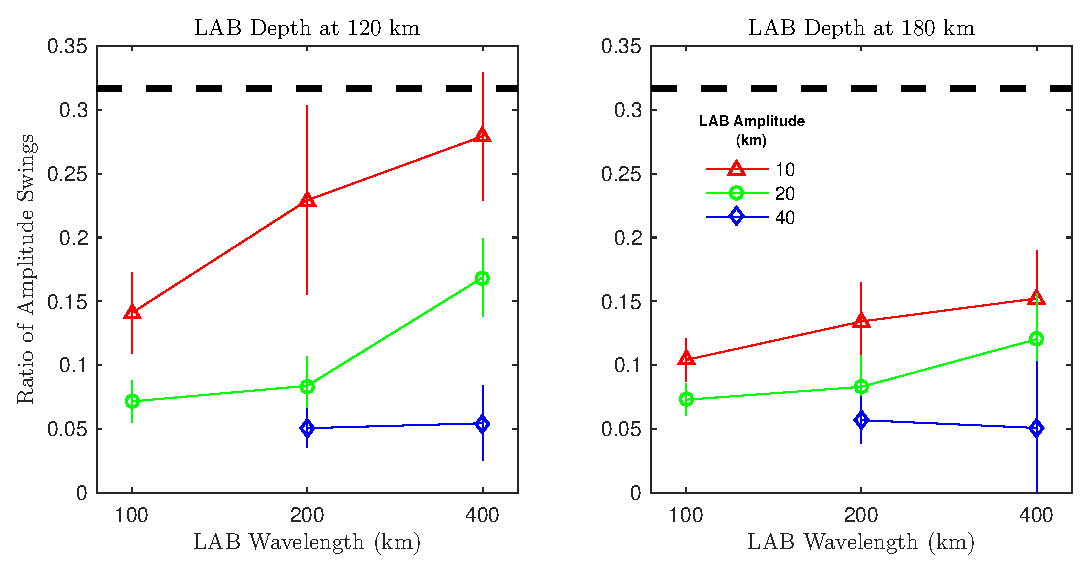
\includegraphics[scale=0.75]{img/FigureRecovery.eps}
\caption{LAB/Moho converter brightness ratio from back-projection results compared to the ratio of LAB and Moho velocity contrasts in the velocity models used to generate the synthetic waveforms (dashed black lines).  The colored symbols mark the ratios of the median values for the LAB and Moho in a given model. The median values for each discontinuity reflect amplitude contrasts taken from the collection of columns from offsets of 1320--2125 in each image.  The vertical lines represent $\pm$ one standard deviation from the median.}
\label{fig:FigureRecovery}
\end{figure}


\label{lastpage}


\end{document}

